\chapter{Electrones en un potencial periódico. Teoría de bandas.} \label{Ch:07}

Para mejorar algunas de las predicciones del modelo del gas de electrones libres se introduce ahora la interacción de los electrones con la red cristalina a través de un potencial periódico. Se sigue despreciando, sin embargo, la posible interacción de los electrones entre sí.

\section{Teorema de Bloch}

Se estudia el comportamiento de un electtón en un potencial con la propiedad $U(\rn)= U(\rn+\Rn)$ siendo $\Rn$ un vector de red. El hecho de que este potencial sea periódico permite establecer la forma general que debe  tener la función de onda. La ecuación de Schrödinger para un electrón es

\begin{equation}  
    - \frac{\hbar^2}{2m} \nabla^2 \Psi (\rn) + U(\rn) \Psi (\rn) = \varepsilon \Psi (\rn) \label{Ec:07-01-01}
\end{equation}
Supongamos el nivel $\varepsilon$ no degenerado (aunque el resultado final no dependa de esta circunstancia). El hecho de que $\Psi (\rn+ \Rn)$ sea también solución de (\ref{Ec:07-01-01}) exige a la función ser igual que $\Psi(\rn)$ salvo por una constante (que puede ser compleja) $\Psi (\Rn+\rn)=C(\Rn) \Psi (\rn)$. Como $\Psi(\rn)$ y $\Psi (\rn + \Rn)$ deben estar normalizadas, se tiene que $|C|^2 = 1 \rightarrow C(\Rn)=e^{i \phi(\Rn)}$. Para dos traslaciones sucesivas $C(\Rn) C(\Rn') = C(\Rn+\Rn')$, que se verifica si $\phi(\Rn)=\kn \cdot \Rn$ donde $\kn$ es un vector constante. En resumen, para cualquier nivel $\varepsilon$ las autofunciones verifican 

\begin{eqnarray}
    \Psi (\rn + \Rn) = e^{i\kn \cdot \Rn} \Psi (\rn) \label{Ec:07-01-02}
\end{eqnarray}
Podemos etiquetar los autoestados por un vector $\kn$ que denominaremos como \textbf{vector de onda}, y entonces $\varepsilon=\varepsilon(\kn)$. Una forma equivalente de (\ref{Ec:07-01-02}) es-nodecimaldot

\begin{eqnarray}
    \Psi (\rn) = u_{\kn} (\rn) e^{i \kn \cdot \rn} \label{Ec:07-01-03}
\end{eqnarray}
donde $u_{\kn} (\rn + \Rn) = u_{\kn} (\rn)$. Este resultado se conoce como \textit{teorema de Bloch}. La solución general (función de onda Bloch) es una onda plana modulada en amplitud. Algunas de las consecuencais que se derivan de (\ref{Ec:07-01-03}) son:

\begin{itemize}
    \item $\kn$ está definido en un vector $\Gn$ perteneciente a la red recíproca, pues si $\kn$ verifica (\ref{Ec:07-01-01}) también lo hace $\kn + \Gn$, y por tanto también $\varepsilon(\kn)=\varepsilon (\kn + \Gn)$. 
    \item La combinación $\hbar \kn$, denominada cuasiimpulso no es el impulso del electrón, pues $i\hbar \nabla \Psi_{\kn} \neq \hbar \kn \Psi_{\kn}$, lo que es consistente pues el impulso no debe ser una constante de movimiento en un potencial periódico.
    \item Por ser hamiltoniano hermítico se puede probar que $\varepsilon(\kn)=\varepsilon(-\kn)$.
    \item Se verifica $|\Psi (\rn) |^2 = |\Psi (\rn + \Rn)|^2$, como debe ser en una estructura periódica.
    \item Al imponer las condiciones de contorno periódicas, los valores de $\kn$ distintos (en una celda primitiva de la red recíproca) son los mismos ya vistos en el Capítulo anterior, esto es, igual al número $N$ de celdas primitvas de la red directa.
\end{itemize}

\section{Aproximación de red vacía}


Se trata de ver los cambios que introduce un potencial periódico (``red'') tan débil que no afecte apreciablemente al espectro de energías del electrón libre:

\begin{equation}
    \varepsilon (\kn) \approx \varepsilon_0 (\kn) \equiv \frac{\hbar^2 k^2}{2m}
\end{equation}
de ahí lo de ``vacía''. En la discusión supondremos 1D para simplificar. Como $\varepsilon(k) = \varepsilon(k+G)$, la relación de dispersión sería la representada en la figura \ref{Fig:07-01} (arriba). Esta reprsentación se denomina \textit{esquema en zona periódica}. Obsérvese que si contamos las porciones de las distintas parábolas que entran en la PZB ya se contabilizan todas las soluciones posibles ($\varepsilon(k)$) de la partícula libre. Se tiene así el llamado \textit{esquema en zona reducida}, representado en la figura \ref{Fig:07-01} (abajo izquierda), donde se ve claro la existencia de mcuhas soluciones para cada valor de $k$. En concreto, todas las energías se pueden representar por 

\begin{equation}
    \varepsilon_0 (k_{PZB}) = \frac{\hbar^2 (k_{PZB}-G)^2}{2m}
\end{equation}
para los distintos $G$ de la red recíproca. Los valores posibles de energía se clasfiican en \textit{bandas de energías}. Así como en este caso todas las energías son posibles, veremos que la presencia de un potencial periódico no despreciable puede introducir intervalos prohibidos de energía entre las diferentes bandas (de ahí toma sentido el concepto de \textit{banda de energía}). Una última reprsentación

\begin{figure}[h!] \centering
    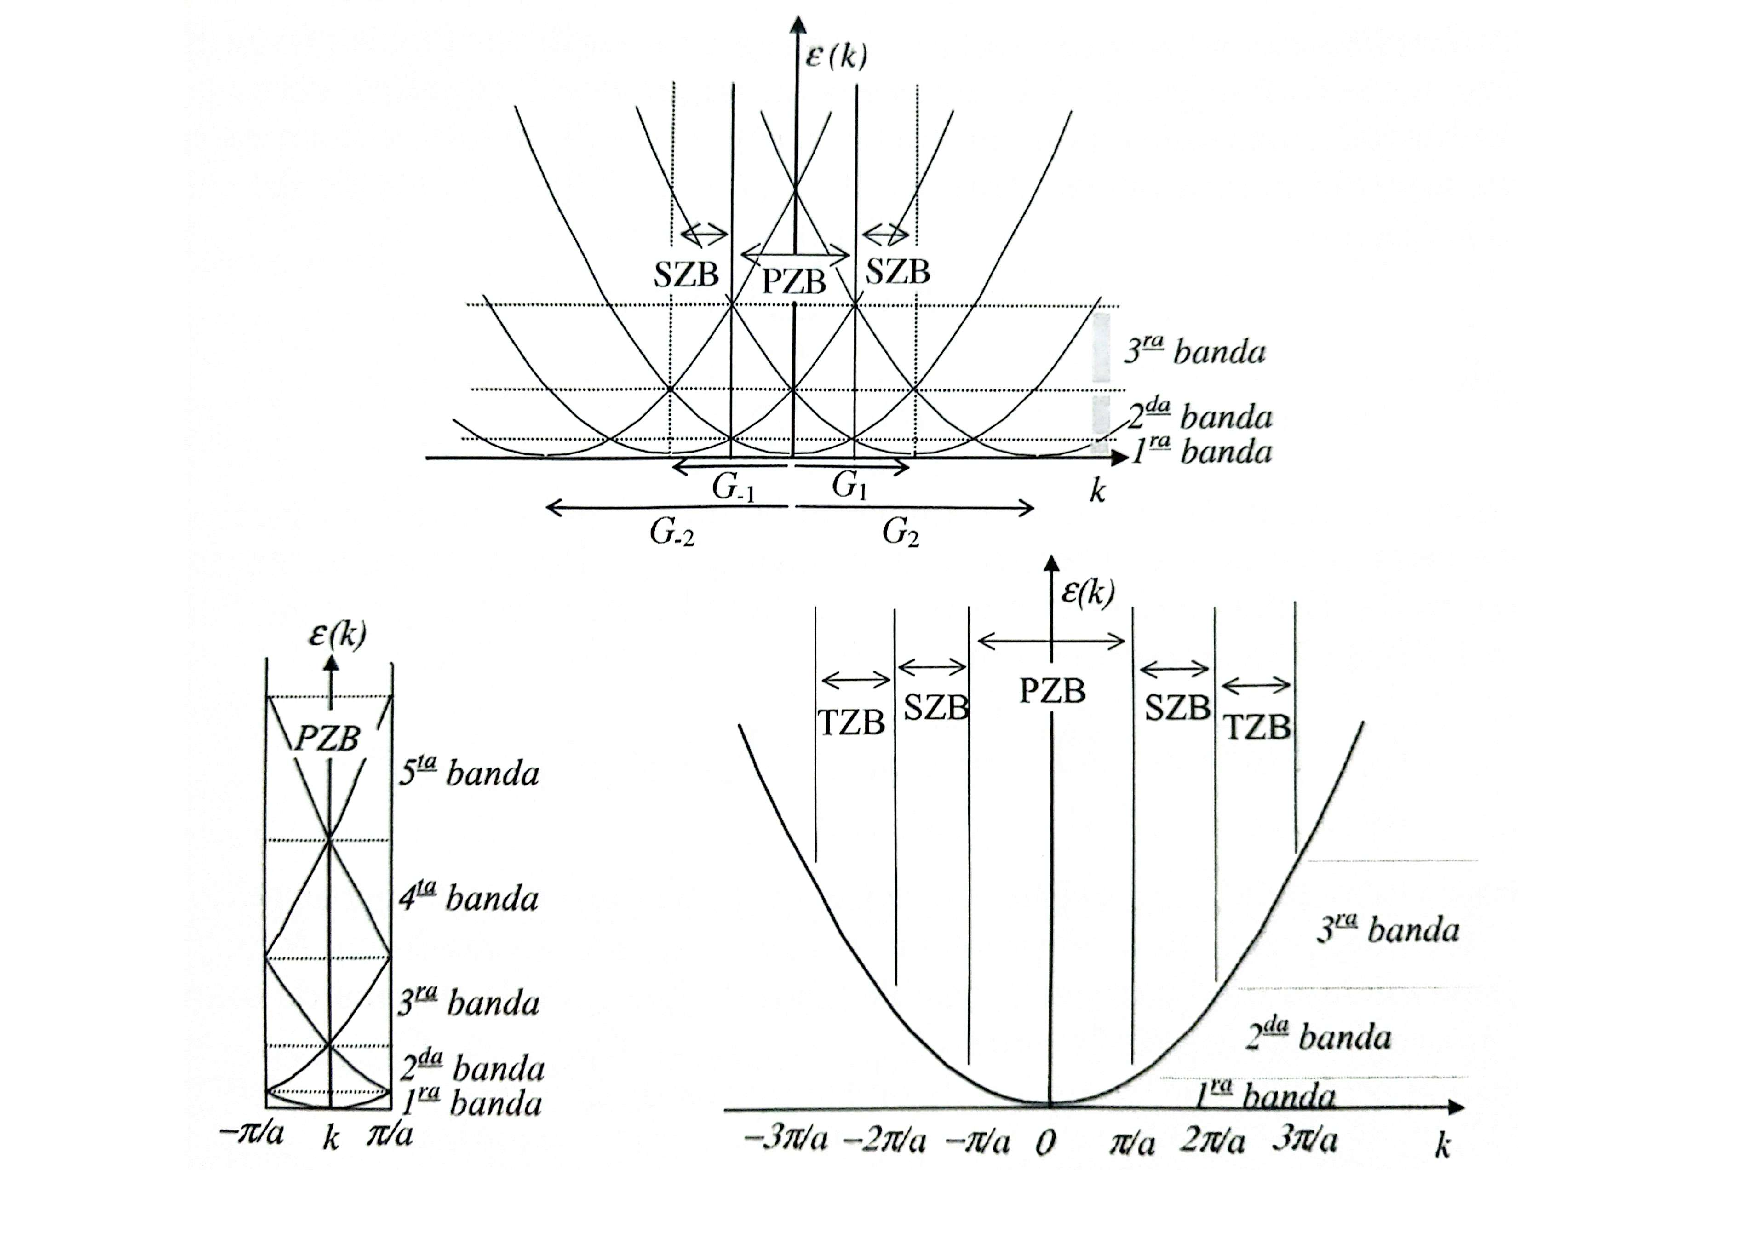
\includegraphics[scale=0.5]{Cuerpo/Ch_07/Fotos libro 1.pdf}
    \caption{Arriba: Esquema en zona periódica. Abajo: Esquemas en zona reducida (izquierda) y en zona extendida (derecha).}
    \label{Fig:07-01}
\end{figure}    



\section{Ecuación de onda del electrón en un potencial periódico}

\section{Electrones cuasilibres}

\subsection{Gap de energía en los bordes de zona}
\begin{figure}[h!] \centering
    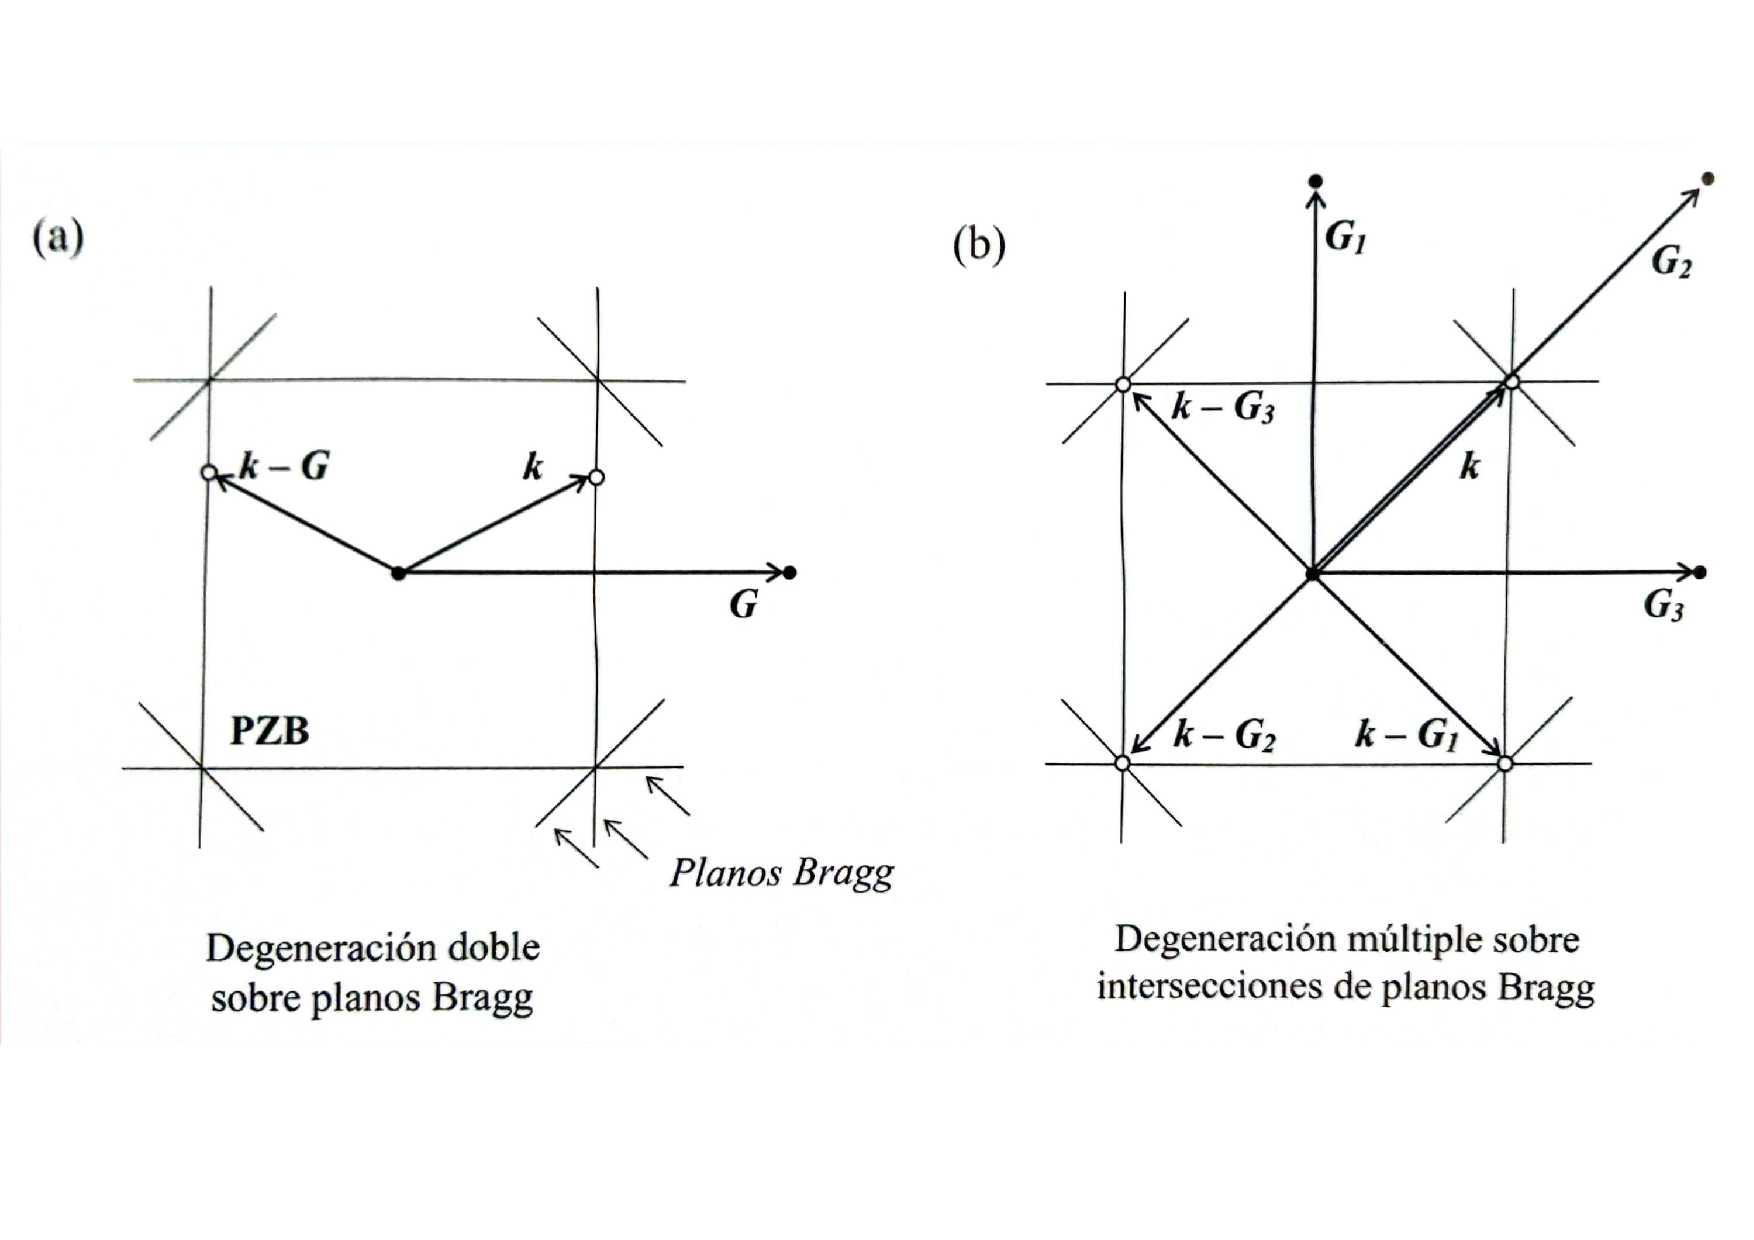
\includegraphics[scale=0.5]{Cuerpo/Ch_07/Fotos libro 2.pdf}
    \caption{(a) Ejemplo de estados doblemente degenerados sobre planos Bragg de una red cuadrada. (b) Estados cuádruplemente degenerados sobre las esquinas de la PZB de una red cuadrada.}
    \label{Fig:07-02}
\end{figure}    

\begin{figure}[h!] \centering
    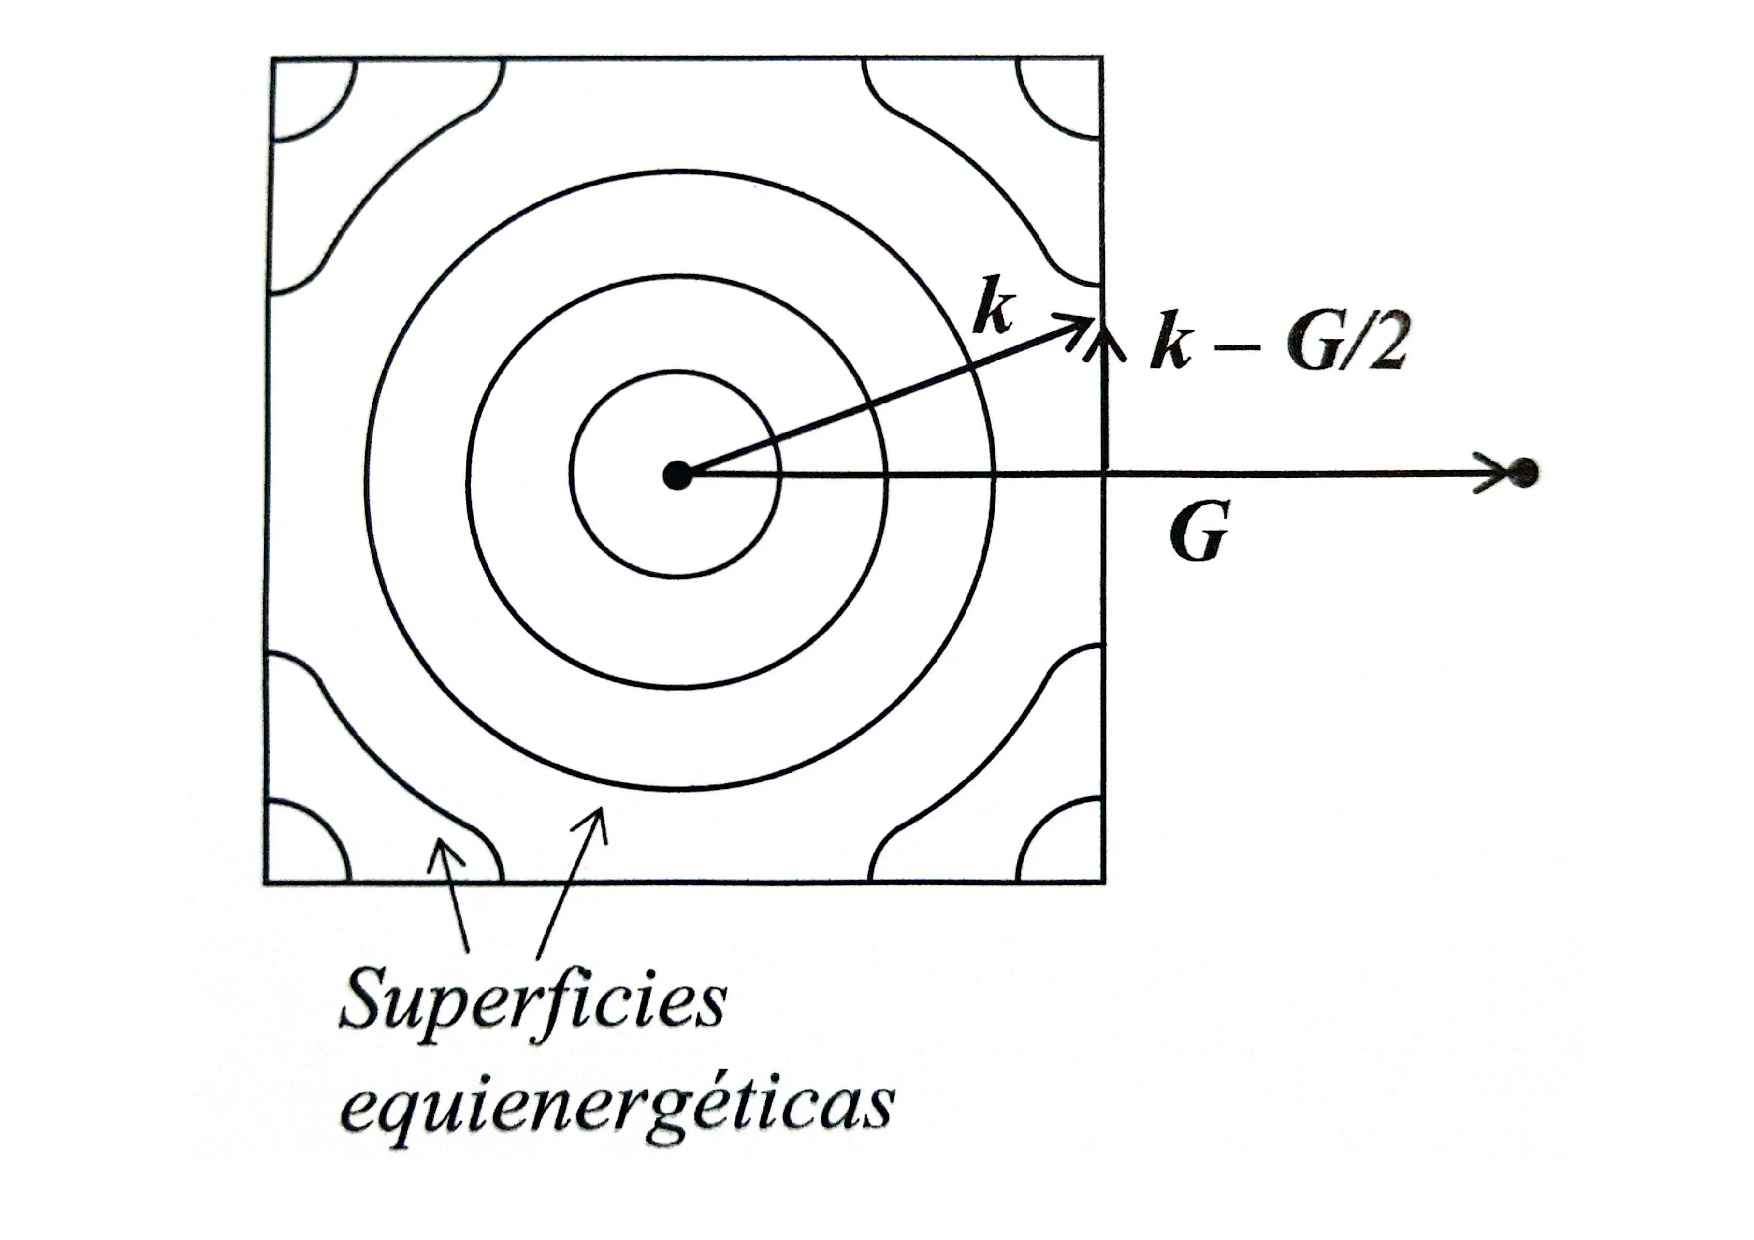
\includegraphics[scale=0.5]{Cuerpo/Ch_07/Fotos libro 3.pdf}
    \caption{Ejemplo de contornos equienergéticos en la PZB de una redcuadrada en la aproximación de electrones cuasilibres. Lejos de los planos de Bragg la aproximación de electrones libres es buena y los contornos son circulares. En los planos de Bragg, según se abre un gap de amplitud $2|U_{\Gn}|$. Según los contornos son perpendiculares a los planos de Bragg.}
    \label{Fig:07-03}
\end{figure}    

\begin{figure}[h!] \centering
    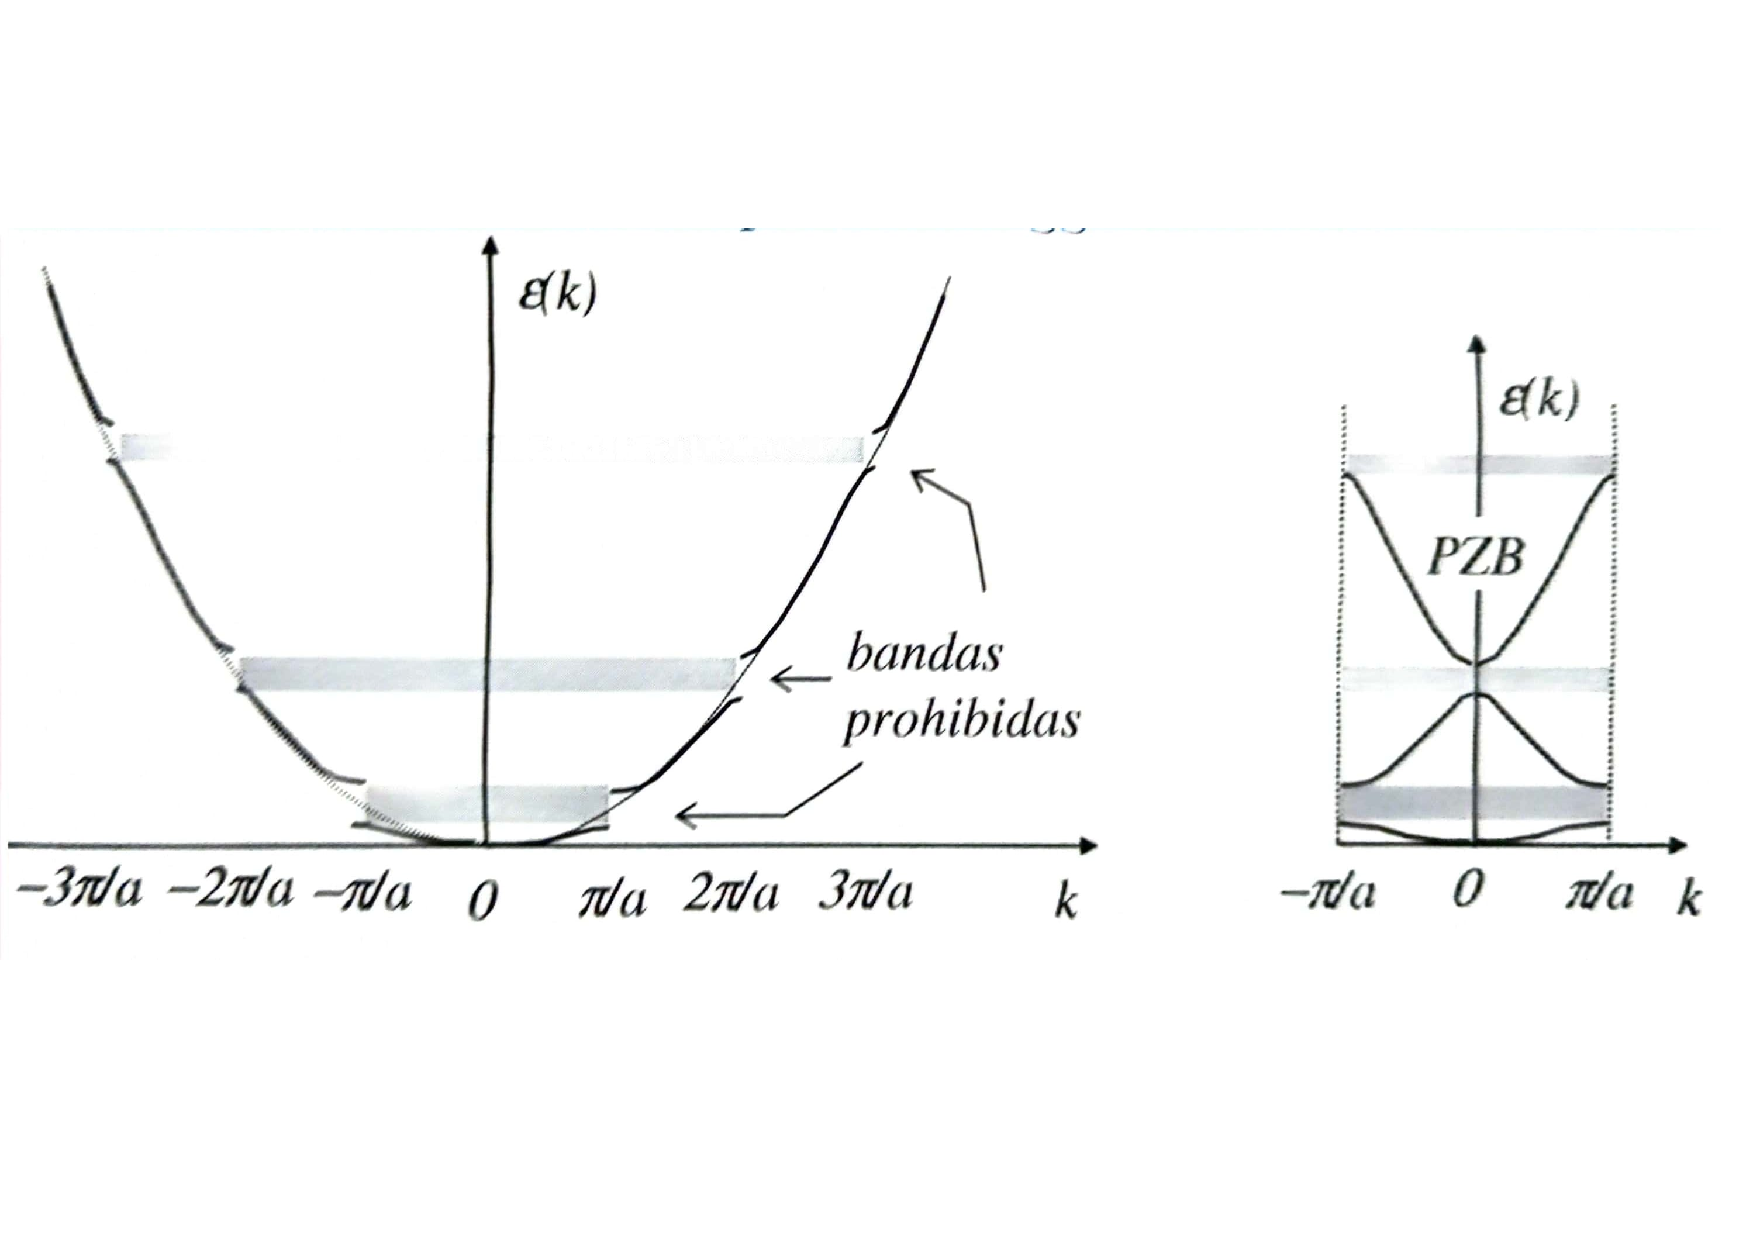
\includegraphics[scale=0.5]{Cuerpo/Ch_07/Fotos libro 4.pdf}
    \caption{Bandas prohibidas en los esquemas en zona extendida (izquierda) y reducida (derecha).}
    \label{Fig:07-04}
\end{figure}    

\section{Electrones fuertemente ligados}

\begin{figure}[h!] \centering
    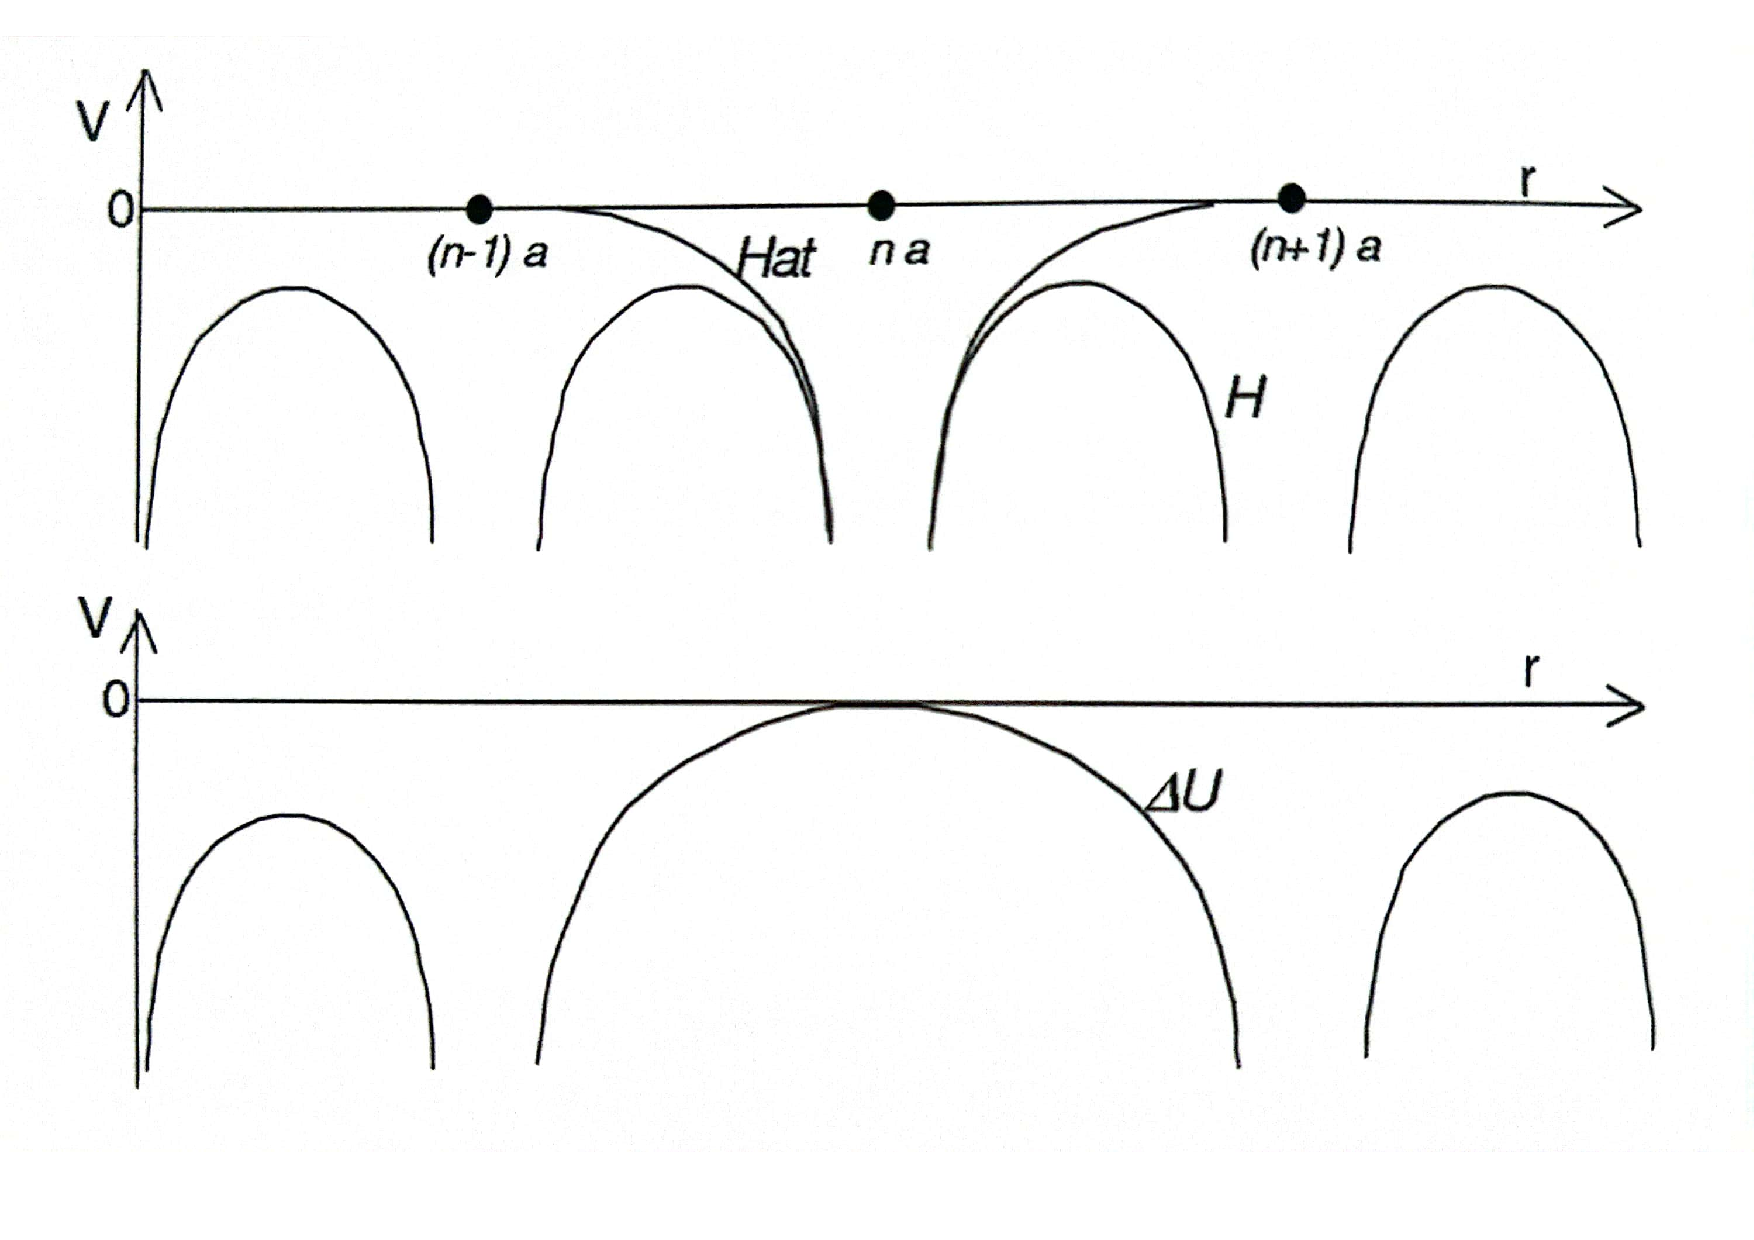
\includegraphics[scale=0.5]{Cuerpo/Ch_07/Fotos libro 5.pdf}
    \caption{Potencial periódico expresado como suma de un potencial atómico más una perturbación.}
    \label{Fig:07-05}
\end{figure}    
\begin{figure}[h!] \centering
    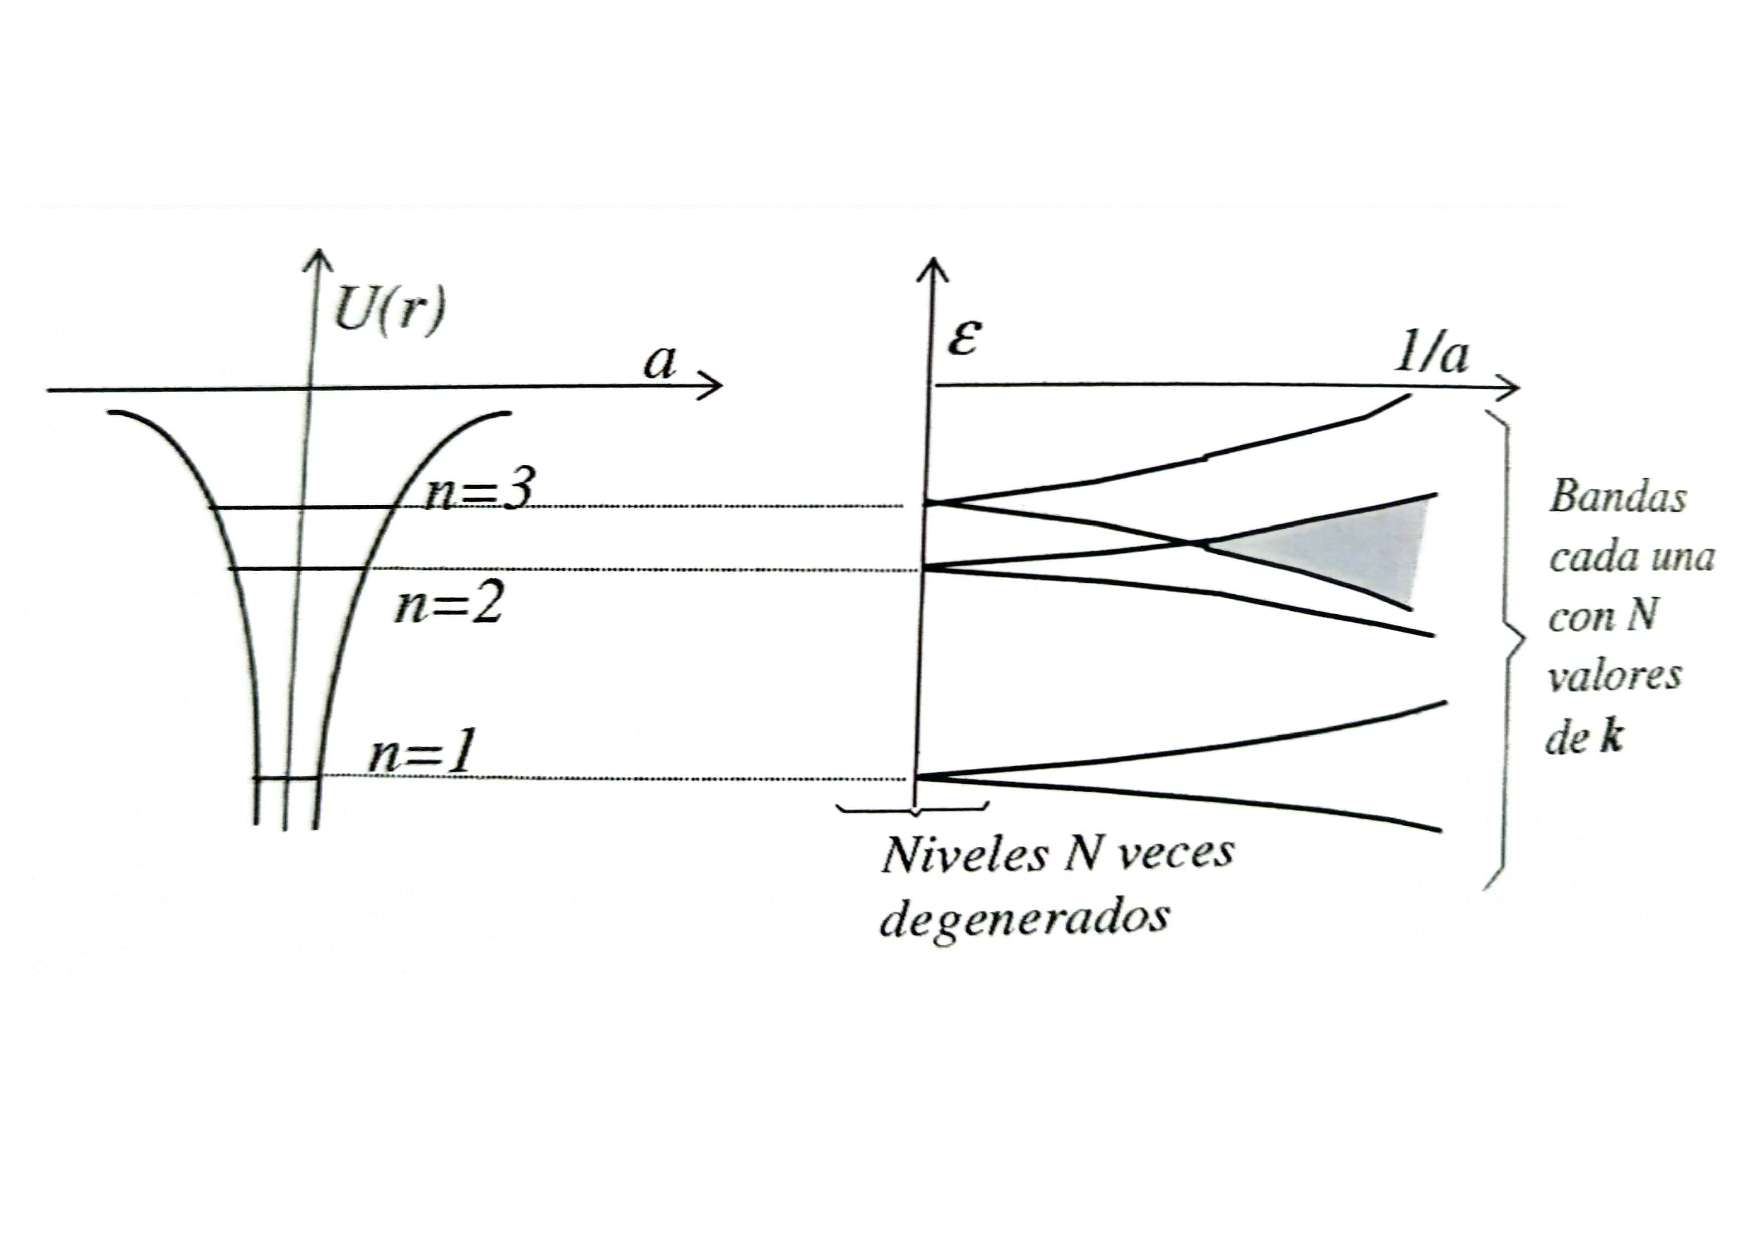
\includegraphics[scale=0.5]{Cuerpo/Ch_07/Fotos libro 6.pdf}
    \caption{Bandas de energía a partir de la aproximación de electrones fuertemente ligados. La zona sombreada representa el solapamiento entre la 1ª y 2ª bandas.}
    \label{Fig:07-06}
\end{figure}    

\section{Superficie de Fermi y zonas de Briollouin}
\begin{figure}[h!] \centering
    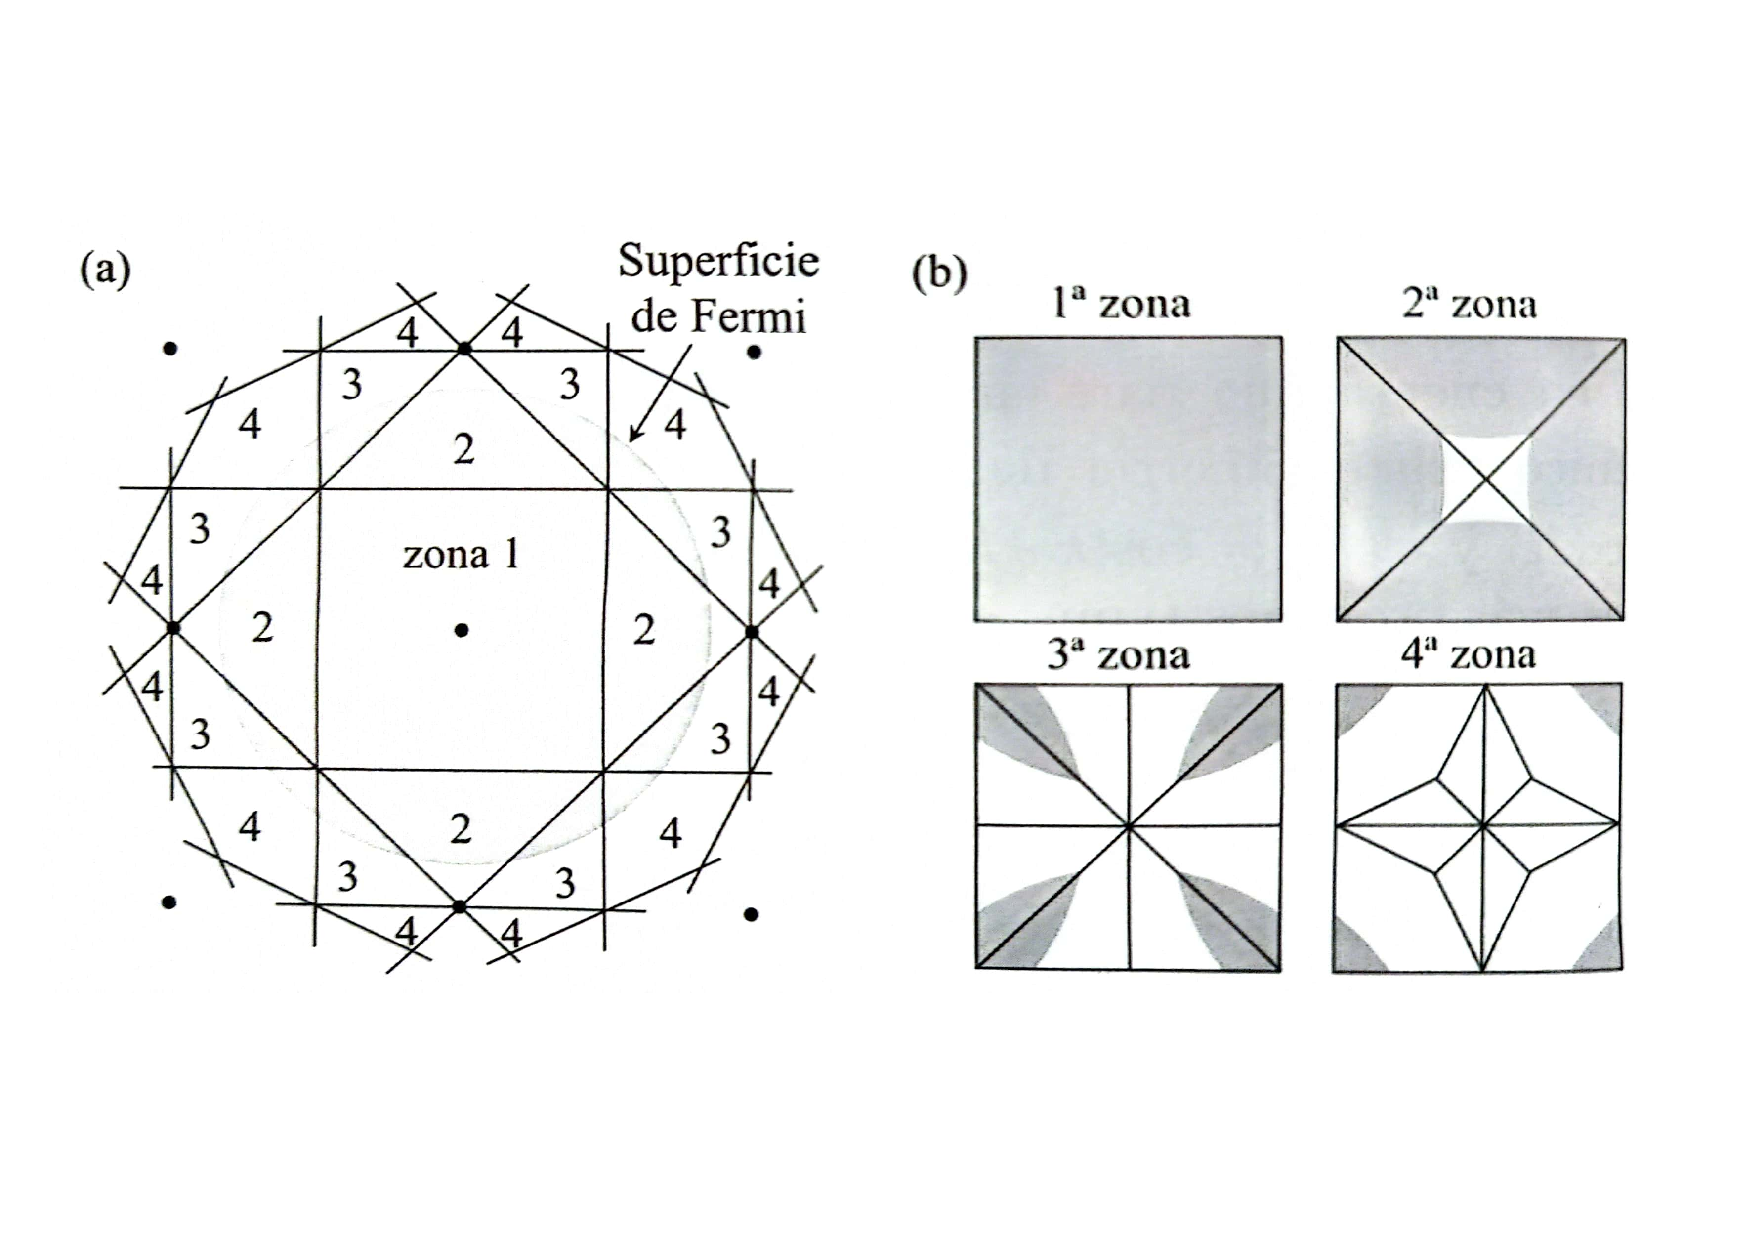
\includegraphics[scale=0.5]{Cuerpo/Ch_07/Fotos libro 7.pdf}
    \caption{1ª, 2ª, 3ª y 4ª zonas de Brillouin para una red cuadrada 2D, según los esquemas en zona extendida (a) y reducida (b). En gris se representan los estados ocupados.}
    \label{Fig:07-07}
\end{figure}    
\begin{figure}[h!] \centering
    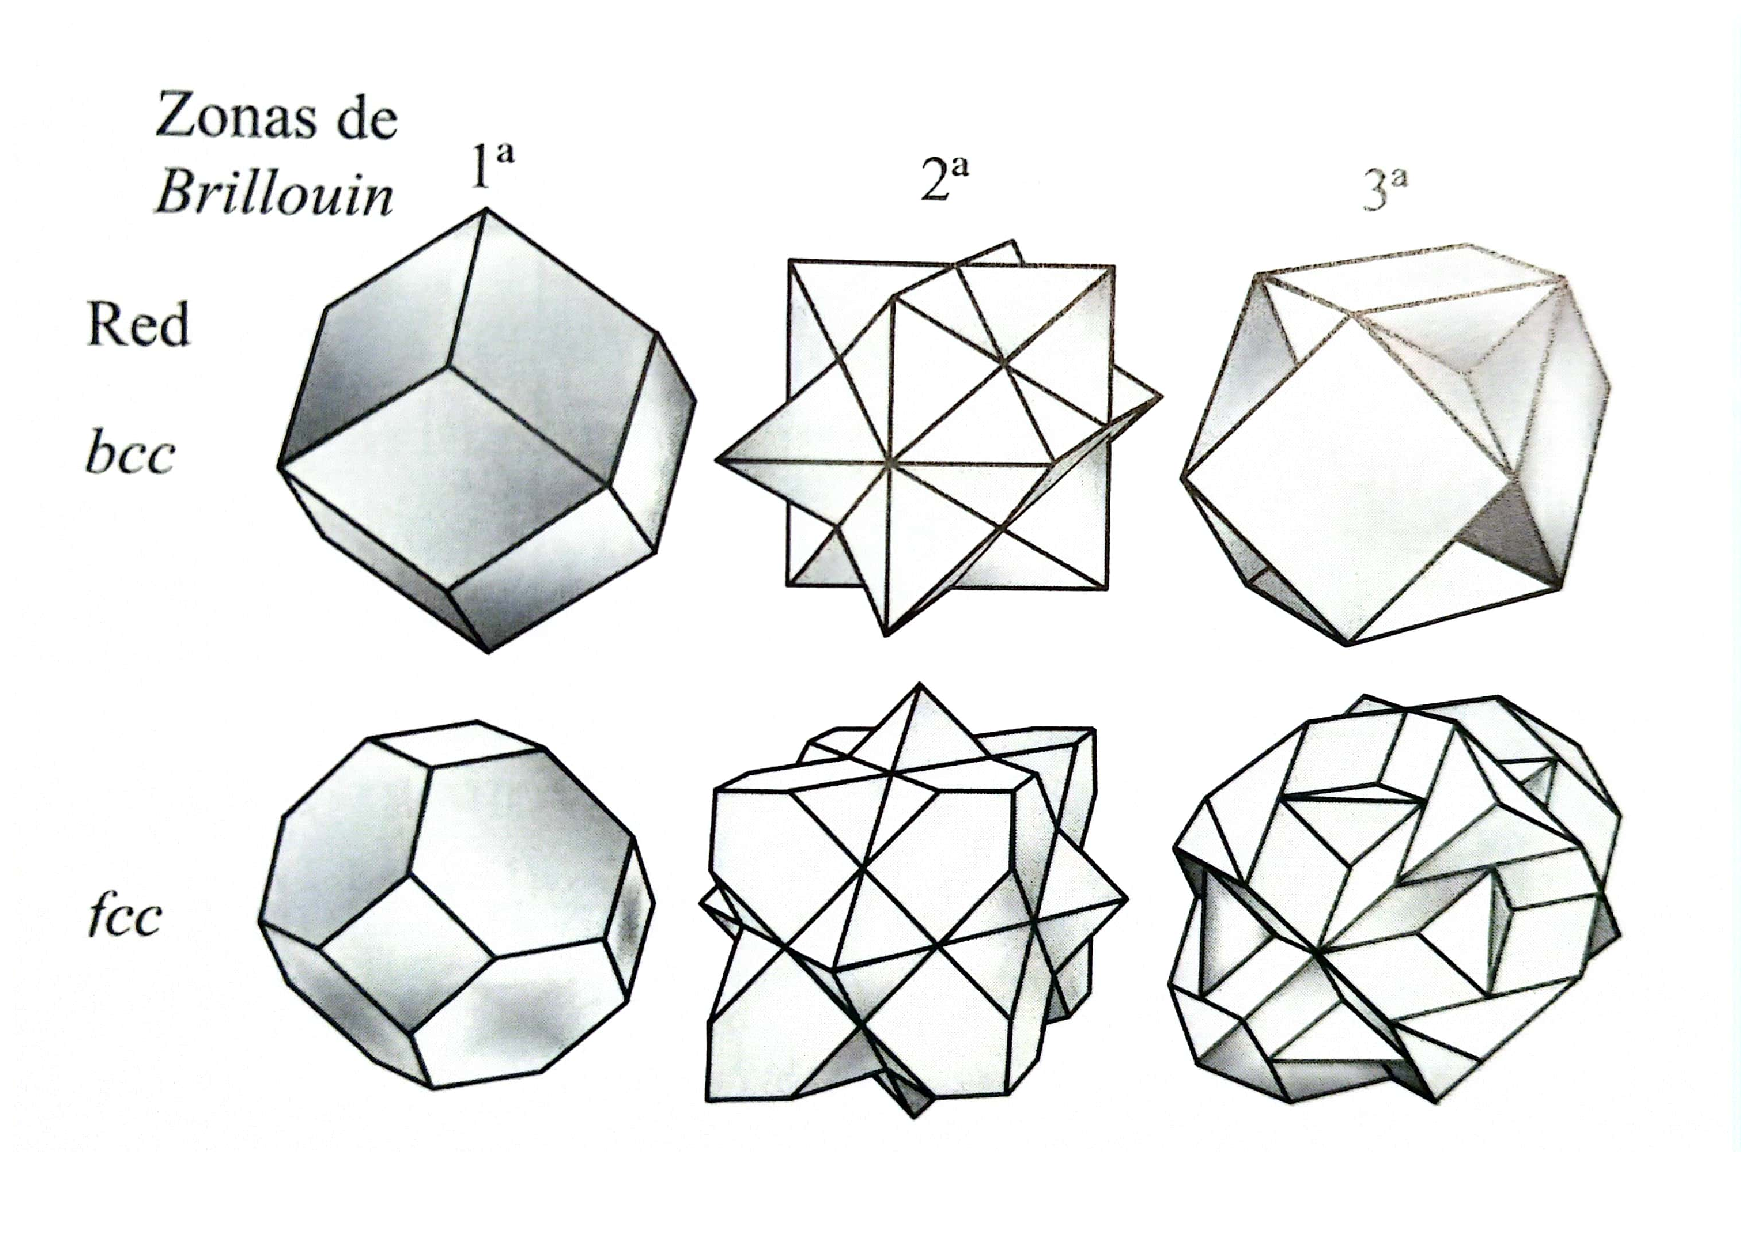
\includegraphics[scale=0.5]{Cuerpo/Ch_07/Fotos libro 8.pdf}
    \caption{Primeras zonas de Brillouin para las estructuras \bcc y \fcc, según el esquema en zona reducida.}
    \label{Fig:07-08}
\end{figure}    
\begin{figure}[h!] \centering
    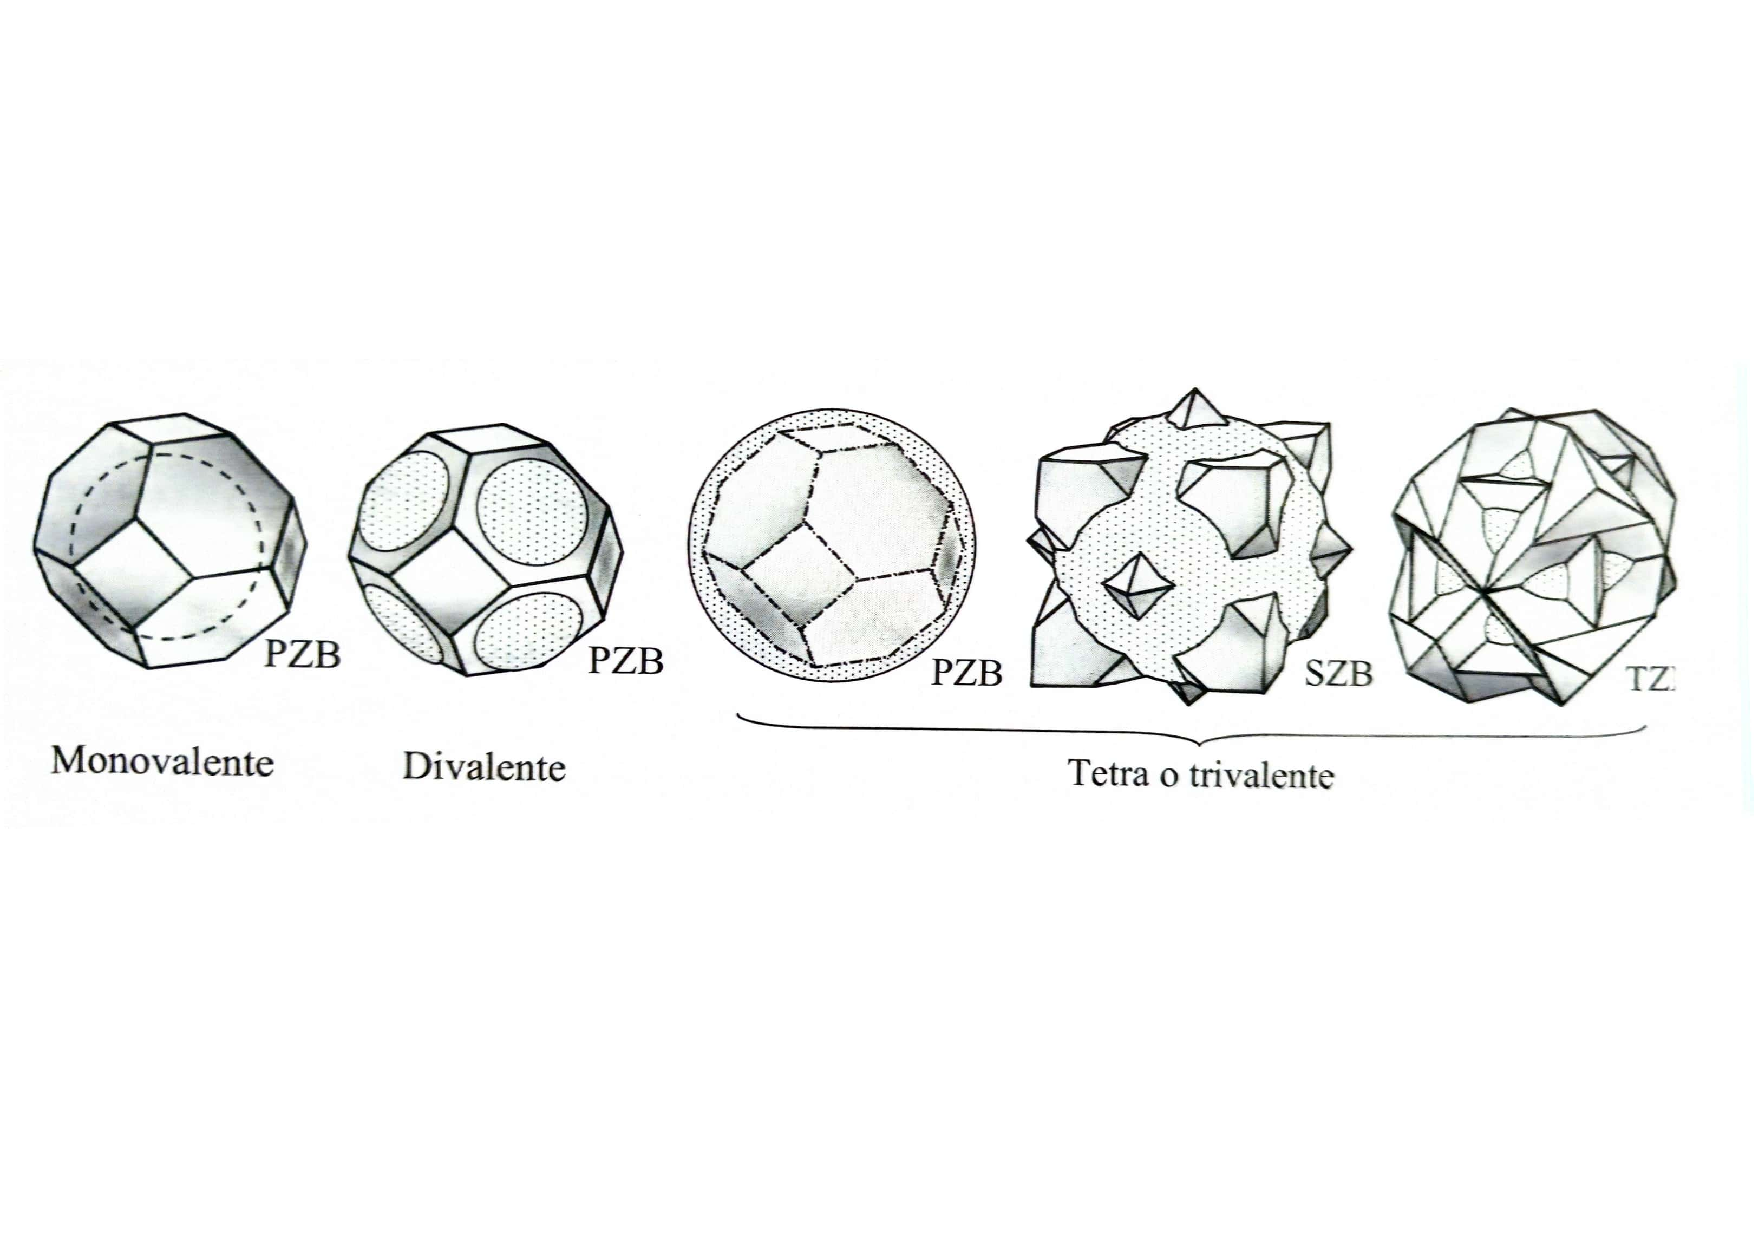
\includegraphics[scale=0.5]{Cuerpo/Ch_07/Fotos libro 9.pdf}
    \caption{Relación entre las primeras zonas de Brillouin de la estructura \fcc y la superficie de Fermi de electrones libres (esférica), según la valencia atómica.}
    \label{Fig:07-09}
\end{figure}    


\section{Metales, aislantes y semiconductores}
\begin{figure}[h!] \centering
    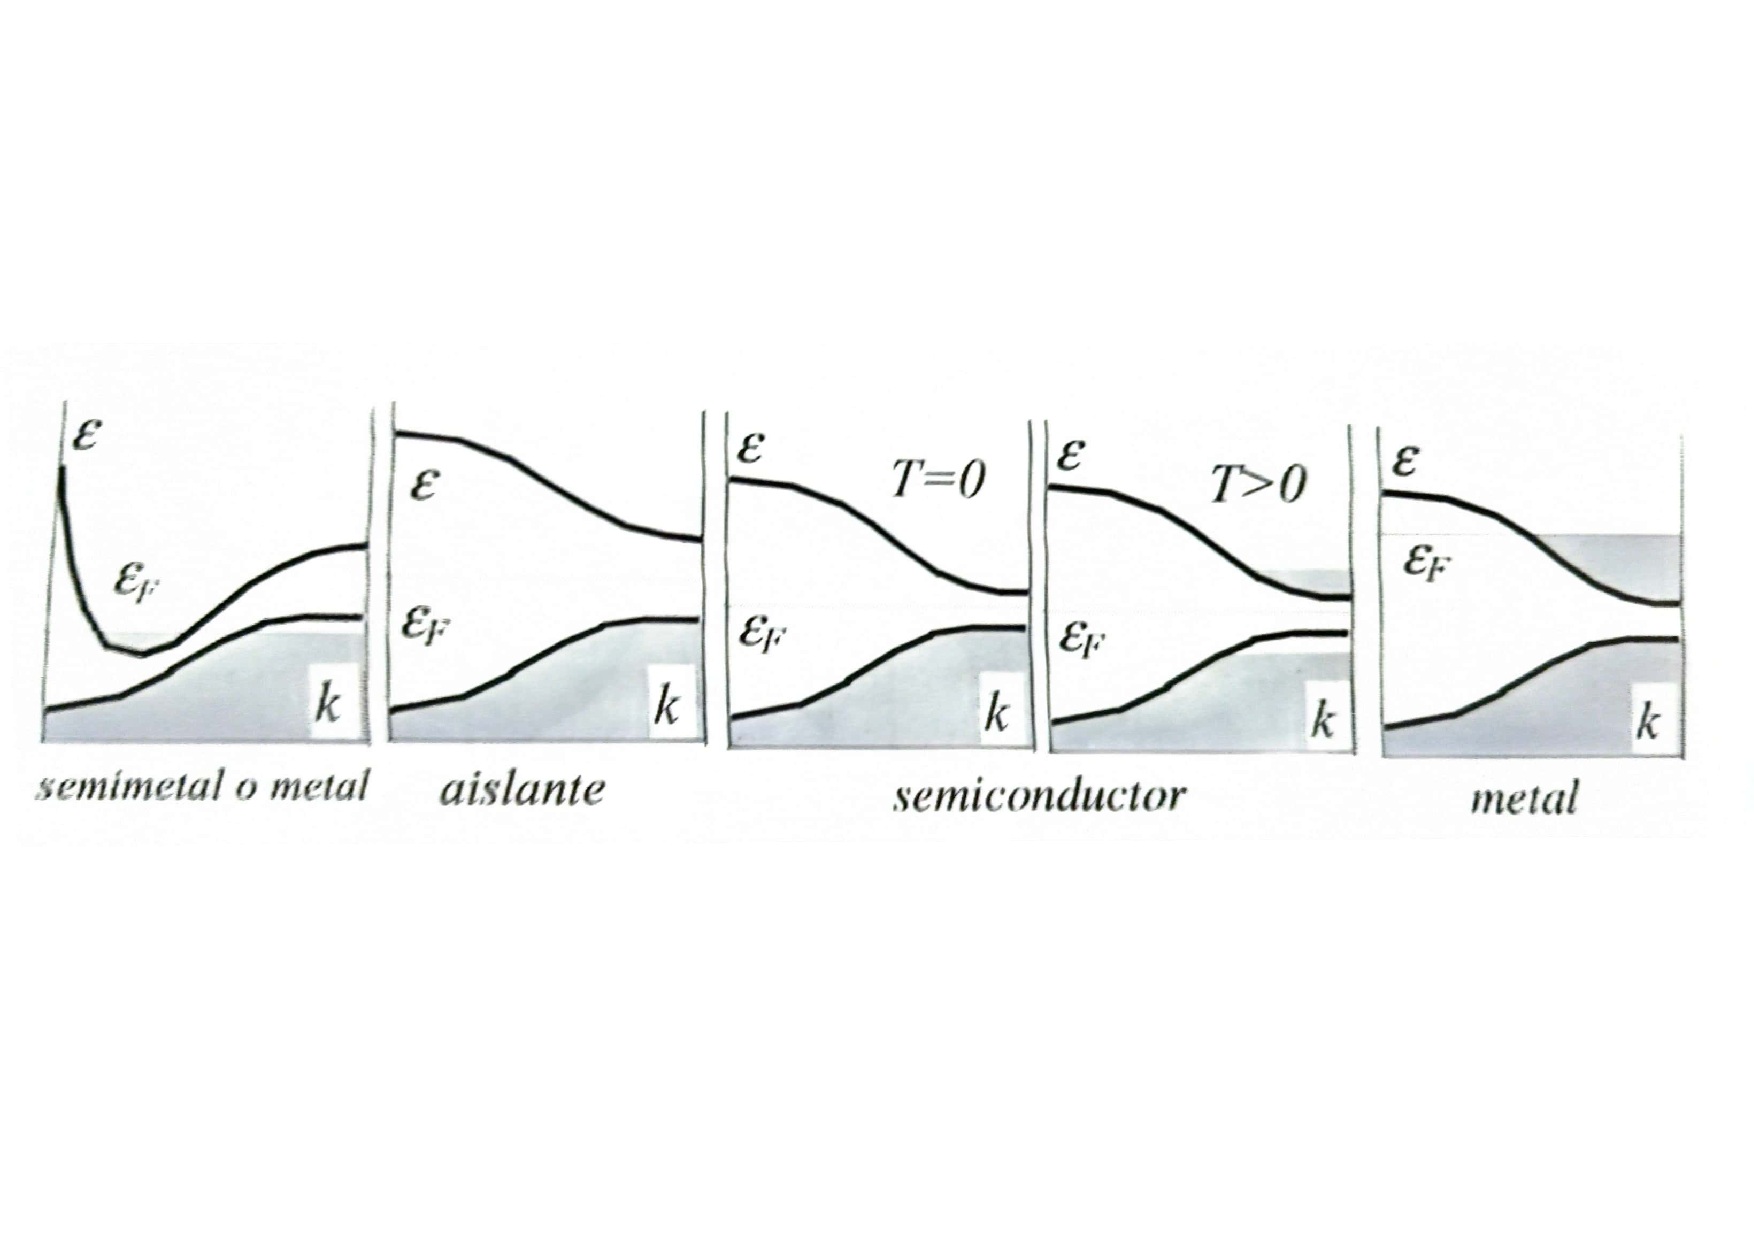
\includegraphics[scale=0.5]{Cuerpo/Ch_07/Fotos libro 10.pdf}
    \caption{Clasifiación de los sólidos según la relación que hay entre el nivel de Fermi y la estructura de bandas.}
    \label{Fig:07-10}
\end{figure}    
